
\PARstart There is strong interest in the development of distributed video analysis
systems that can be used to analyze large video databases. Unfortunately, the
overwhelming majority of software packages for automated video analysis, are not
necessarily designed to scale  to handle processing  vast video
databases.

An example of a large-scale video database is  provided by the advancing out of
school learning in mathematics and engineering (AOLME) project. AOLME contains
over a thousand hours of high quality video data that need to be analyzed so as
to understand how middle school students acquire basic programming skills.
Currently, most of this analysis is done manually \cite{LopezLeiva2016} to
extract pertinent features for researchers to analyze, which is an extremely
labor intensive job and thus leaves many of the videos unanalyzed. Clearly
there is a need for a tool researchers of education can leverage to
more successfully analyze their subjects.

Current methods in video analysis systems are extremely application dependent
and are inadequate computationally to sufficiently
investigate video datasets at such a large scale. As such, there is a propensity
for a system that is accurate, scalable and flexible in nature to handle a
variety of challenges in automated video analysis. Not only this, but the system
should be able to leverage computational success in the vertical and horizontal
architectures.

% Computationally, there is clearly a need for video analysis methods that can be
% efficiently implemented in heterogenous compute hardware (such as GPUS and
% CPUS), and have said hardware function in a distributed environment. Being able
% to leverage heterogenous computer hardware greatly increases the efficiency and
% speed of certain, heavily used, video processing algorithms such as 2D
% convolutions. Furthermore, having this system exist in a distributed environment
% will greatly speed up ephemeral operations and makes it possible to scale up to
% address large scale problems. Thus this paper is motivated by the challenges
% associated with analyzing large scale video databases.

% The human activities that are considered as part of this research are
% illustrated in Figure \ref{fig:typing_writing}. We explore the problem
% of classifying typing versus no-typing and writing versus no-writing using
% optical flow methods.

The proposed research represents a novel extension of prior research undertaken
at the image and video processing and communications laboratory. Prior efforts
focused on the development AM-FM representations \cite{5378645} \cite{Cesar2012}
\cite{6693707} \cite{loizou2014despeckle} \cite{agurto2011automatic}
\cite{5590295} \cite{5414522} \cite{5405648} \cite{murray2012} \cite{4135672}
\cite{908521} \cite{765139} \cite{janakiramanan2011tree} \cite{985561}
\cite{931092} \cite{923291} \cite{758405} and the development of dynamically
reconfigurable architectures \cite{Carranza2016} \cite{llamocca2014dynamic}
\cite{7418203} \cite{7015949} \cite{jiang2014dynamically} \cite{6806021}
\cite{6810466}.

In this paper, we show that it is possible to reduce the feature set of videos
on the order of Gigabytes down to tens of Kilobytes, and then accurately
classify those features at very high accuracy as a particular human activity. We
use videos shown in \ref{fig:typing_writing} as our data. We also create an
architecture that is capable of scaling to dozens of compute notes, and
potentially thousands thus making the heavy lifting operations, such as
computing optical flow vectors, a trivial task that can be efficiently performed
in the Amazon Web Services (AWS) cloud, thus enabling researchers to extract
germane features from videos in a matter of minutes instead of hours.
Additionally, all the software provided in this research is released under the
MIT open source license to facilitate further extension of this area.

\begin{figure*}[t]
  \centering
  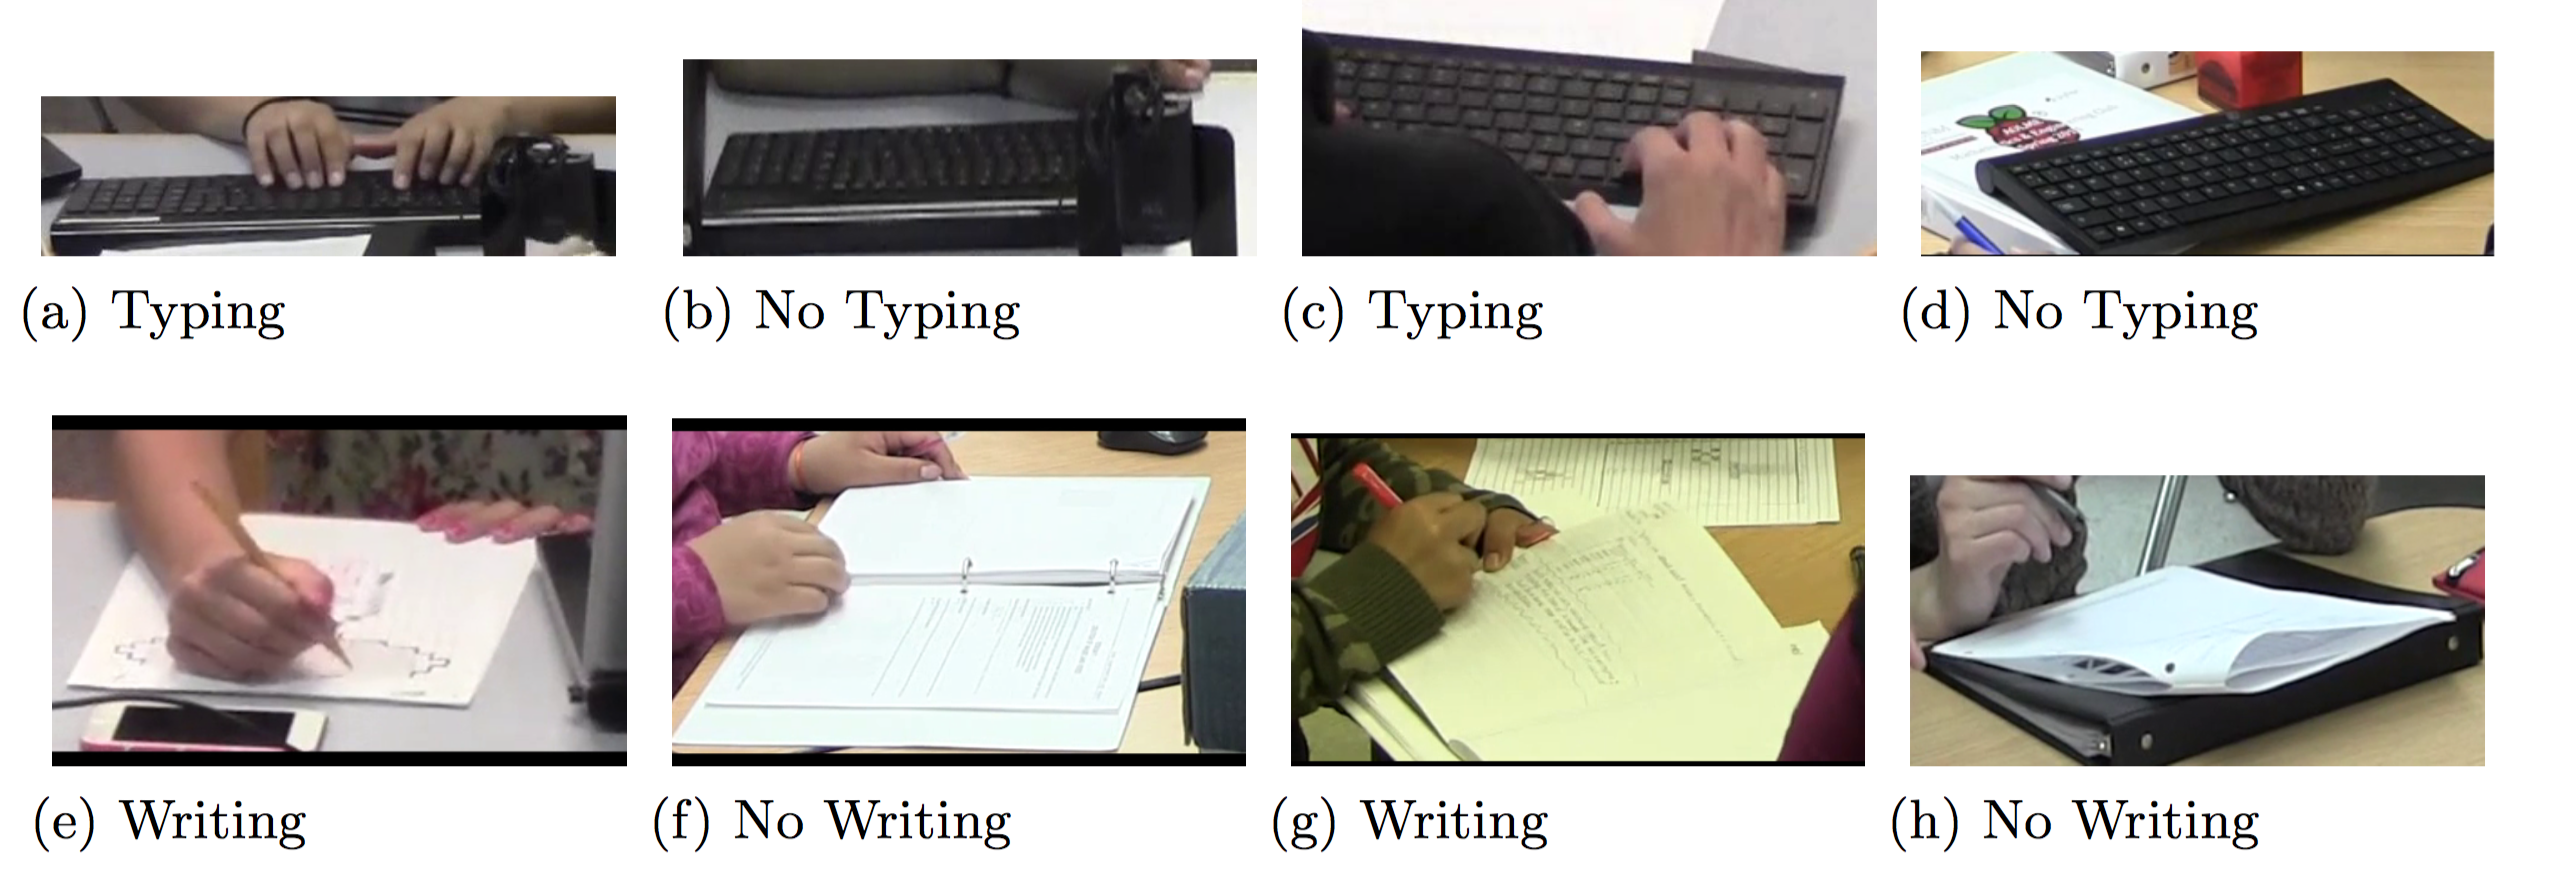
\includegraphics[width=\textwidth]{figures/typing_writing_clip}
  \caption{Example of features that have been manually extracted from the dataset
  for training and testing. For the above example, we need to classifiers for each
  activity to determine if the activity is being performed, or it is not.}
  \label{fig:typing_writing}
\end{figure*}
